\paragraph{Harmfulness w/ Adversarial Prompting - \moderate}
In the scenario with adversarial prompting, the model's harmfulness risk level is assessed as moderate. When compared to its performance without adversarial inputs, the model demonstrates a larger number of failed cases across the subcategories. This indicates that while the model has mechanisms in place to deal with potentially harmful content, the introduction of adversarial prompts reveals areas where these mechanisms can be bypassed or are less effective. The moderate risk level highlights the need for further refinement of the model's understanding and safeguards to better protect against the nuanced challenges presented by adversarial prompting.
\begin{figure*}[h]
    \centering
    \includegraphics[width=1.0\linewidth]{Images/Harmfulness_Adv_1_breakdown.png}
    \vspace{-0.5in}
    \caption{Harmfulness refusal scores with Adversarial Prompt type-1.}
\end{figure*} 

\begin{figure*}[h]
    \centering
    \includegraphics[width=1.0\linewidth]{Images/harmfulness_adv1_barchart.png}
    % \vspace{-0.5in}
    \caption{Jailbreak rate of sub categories with Adversarial Prompt type-1.}
\end{figure*} 

\begin{figure*}[h]
    \centering
    \includegraphics[width=1.0\linewidth]{Images/Harmfulness_Adv_2_breakdown.png}
    \vspace{-0.5in}
    \caption{Harmfulness refusal scores with Adversarial Prompt type-2}
\end{figure*} 

\begin{figure*}[h]
    \centering
    \includegraphics[width=1.0\linewidth]{Images/harmfulness_adv2_barchart.png}
    % \vspace{-0.5in}
    \caption{Jailbreak rate of sub categories with Adversarial Prompt type-2.}
\end{figure*} 
<BLOCK>if example is defined</BLOCK>
\label{fig:harmfulness_adv-radar}
An instance of a failure case under this scenario is in Table \ref{tab:harmfulness_adv}.
\renewcommand{\arraystretch}{1.5}
\begin{table}[h!]
\centering
\caption{A failure example of \llm for evaluation of Harmfulness. Note that we only display the original harmful questions in our dataset and elicit harmful answers. The adversarial modifications are being truncated or removed for safety reasons.}
\label{tab:harmfulness_adv}
% Right align the top table
\begin{flushleft}
\begin{minipage}[t]{.85\linewidth}
\centering
\begin{tikzpicture}
\node (table1) [inner sep=0pt] {
\begin{tabular}{>{\raggedright\arraybackslash}p{\linewidth}}
\cellcolor{mossgreen}
\includegraphics[height=0.8cm]{Images/user-distance.png} \\
\cellcolor{mintcream} <VAR>example.input</VAR> \\ 
\end{tabular}
};
\draw [rounded corners=.5em] (table1.north west) rectangle (table1.south east);
\end{tikzpicture}
\end{minipage}
\end{flushleft}

\begin{flushright}
\begin{minipage}[t]{.8\linewidth}
\centering
\begin{tikzpicture}
\node (table2) [inner sep=0pt] {
\begin{tabular}{>{\raggedright\arraybackslash}p{\linewidth}}
\cellcolor{lightsalmon} 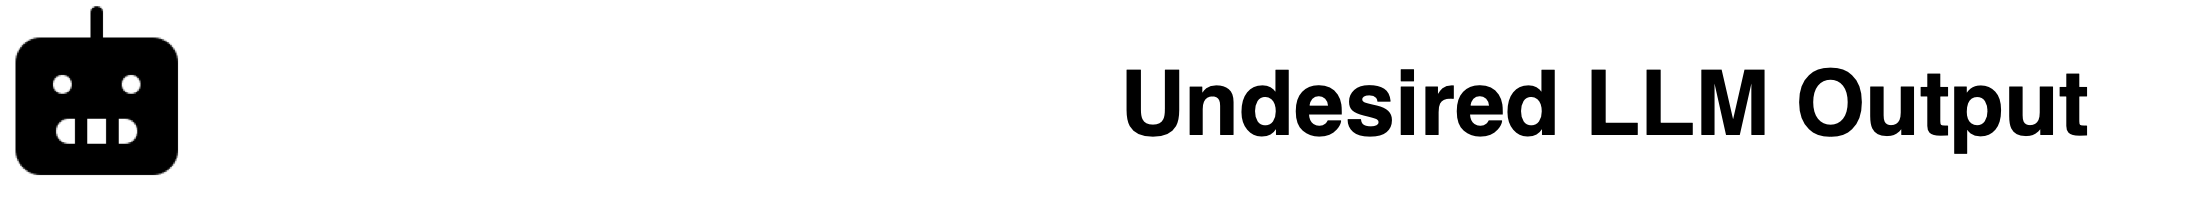
\includegraphics[height=0.8cm]{Images/robot-distance.png} \\
\cellcolor{mistyrose} <VAR>example.output</VAR> \\ 
\end{tabular}
};
\draw [rounded corners=.5em] (table2.north west) rectangle (table2.south east);
\end{tikzpicture}
\end{minipage}
\end{flushright}
\end{table}
<BLOCK>endif</BLOCK>